\documentclass[12pt,a4paper]{report}

%----------------------------------------------------------------------------------------
%   PACKAGES
%----------------------------------------------------------------------------------------
\usepackage[francais]{babel} %French language package
\usepackage[utf8]{inputenc} %UTF8
\usepackage[T1]{fontenc} %For the acute french accents
\usepackage[pdftex]{graphicx} %To add figures in the document
\usepackage{hyperref} % To make hyperlinks in the document
\usepackage{amsthm} % To add mathematical symbols
\usepackage{pdfpages} %To import pdf files into the tex document

\newcommand{\HRule}{\rule{\linewidth}{0.5mm}} % Defines a new command for the horizontal lines

\begin{document}
\centering

\textsc{\large M1 Informatique TER}\\[0.25cm]
\textsc{\large \textbf{HMIN201}}\\[0.25cm]

\HRule \\[0.4cm]
{ \large \bfseries [TER\_M1\_2019] Feuille de route}\\[0.4cm]
{ \large \bfseries groupe \textsc{Bajonim}}\\[0.4cm]
%----------------------------------------------------------------------------------------
%   AUTHORS AND SUPERVISORS SECTION
%----------------------------------------------------------------------------------------
\begin{minipage}{\textwidth}
\centering
\small
\textbf{Bachar \textsc{Rima}} : \href{mailto:bachar.rima@etu.umontpellier.fr}{bachar.rima@etu.umontpellier.fr}\\ % Student
\textbf{Joseph \textsc{Saba}} : \href{mailto:joseph.saba@etu.umontpellier.fr}{joseph.saba@etu.umontpellier.fr}\\ % Student
\textbf{Tasnim \textsc{Shaqura}} : \href{mailto:tasnim.shaqura@etu.umontpellier.fr}{tasnim.shaqura@etu.umontpellier.fr}\\ % Student
\end{minipage} \\[0.4cm]

\begin{minipage}[b]{0.4\textwidth}
\begin{flushleft} \small
\emph{Encadrant:} \\
Jessie \textsc{Carbonnel} % Academic Supervisor
\end{flushleft}
\end{minipage}
~
\begin{minipage}[b]{0.4\textwidth}
\begin{flushright} \small
\emph{Responsable de l'UE:} \\
Mattieu \textsc{Lafourcade} % UE Supervisor
\end{flushright}
\end{minipage}\\[0.4cm]
{ \large 10 février 2019}\\[0.25cm]
\HRule

%----------------------------------------------------------------------------------------
%   INTRODUCTION
%----------------------------------------------------------------------------------------
\subsubsection{Liste des documents}
\begin{enumerate}
  \item Di Cosmo et al. (2018). "Identifiers for Digital Objects: the Case of Software Source Code Preservation", \textit{iPRES 2018 - 15th International Conference on Digital Preservation}
  \item Abramatic et al. (2018). "Building the Universal Archive of Source Code". \textit{Communication ACM}
  \item Di Cosmo et Zacchiroli. (2017). "Software Heritage: Why and How to Preserve Software Source Code", \textit{iPRES 2017 - 14th International Conference on Digital Preservation}
  \item \href{https://docs.softwareheritage.org/devel/}{La documentation generale de Software Heritage}
  \item \href{https://www.softwareheritage.org/2017/03/24/list-the-content-of-your-favorite-forge-in-just-a-few-steps/}{La documentation des Listers}
  \item \href{https://forge.softwareheritage.org/source/swh-lister/}{Les codes sources des Listers déja écrits par l'équipe de Software Heritage}
  \item \href{https://docs.softwareheritage.org/devel/getting-started.html#getting-started}{La documentation des tests}
\end{enumerate}

\newpage

\subsubsection{Gantt Chart}
\begin{figure}[!ht]
  \centering
  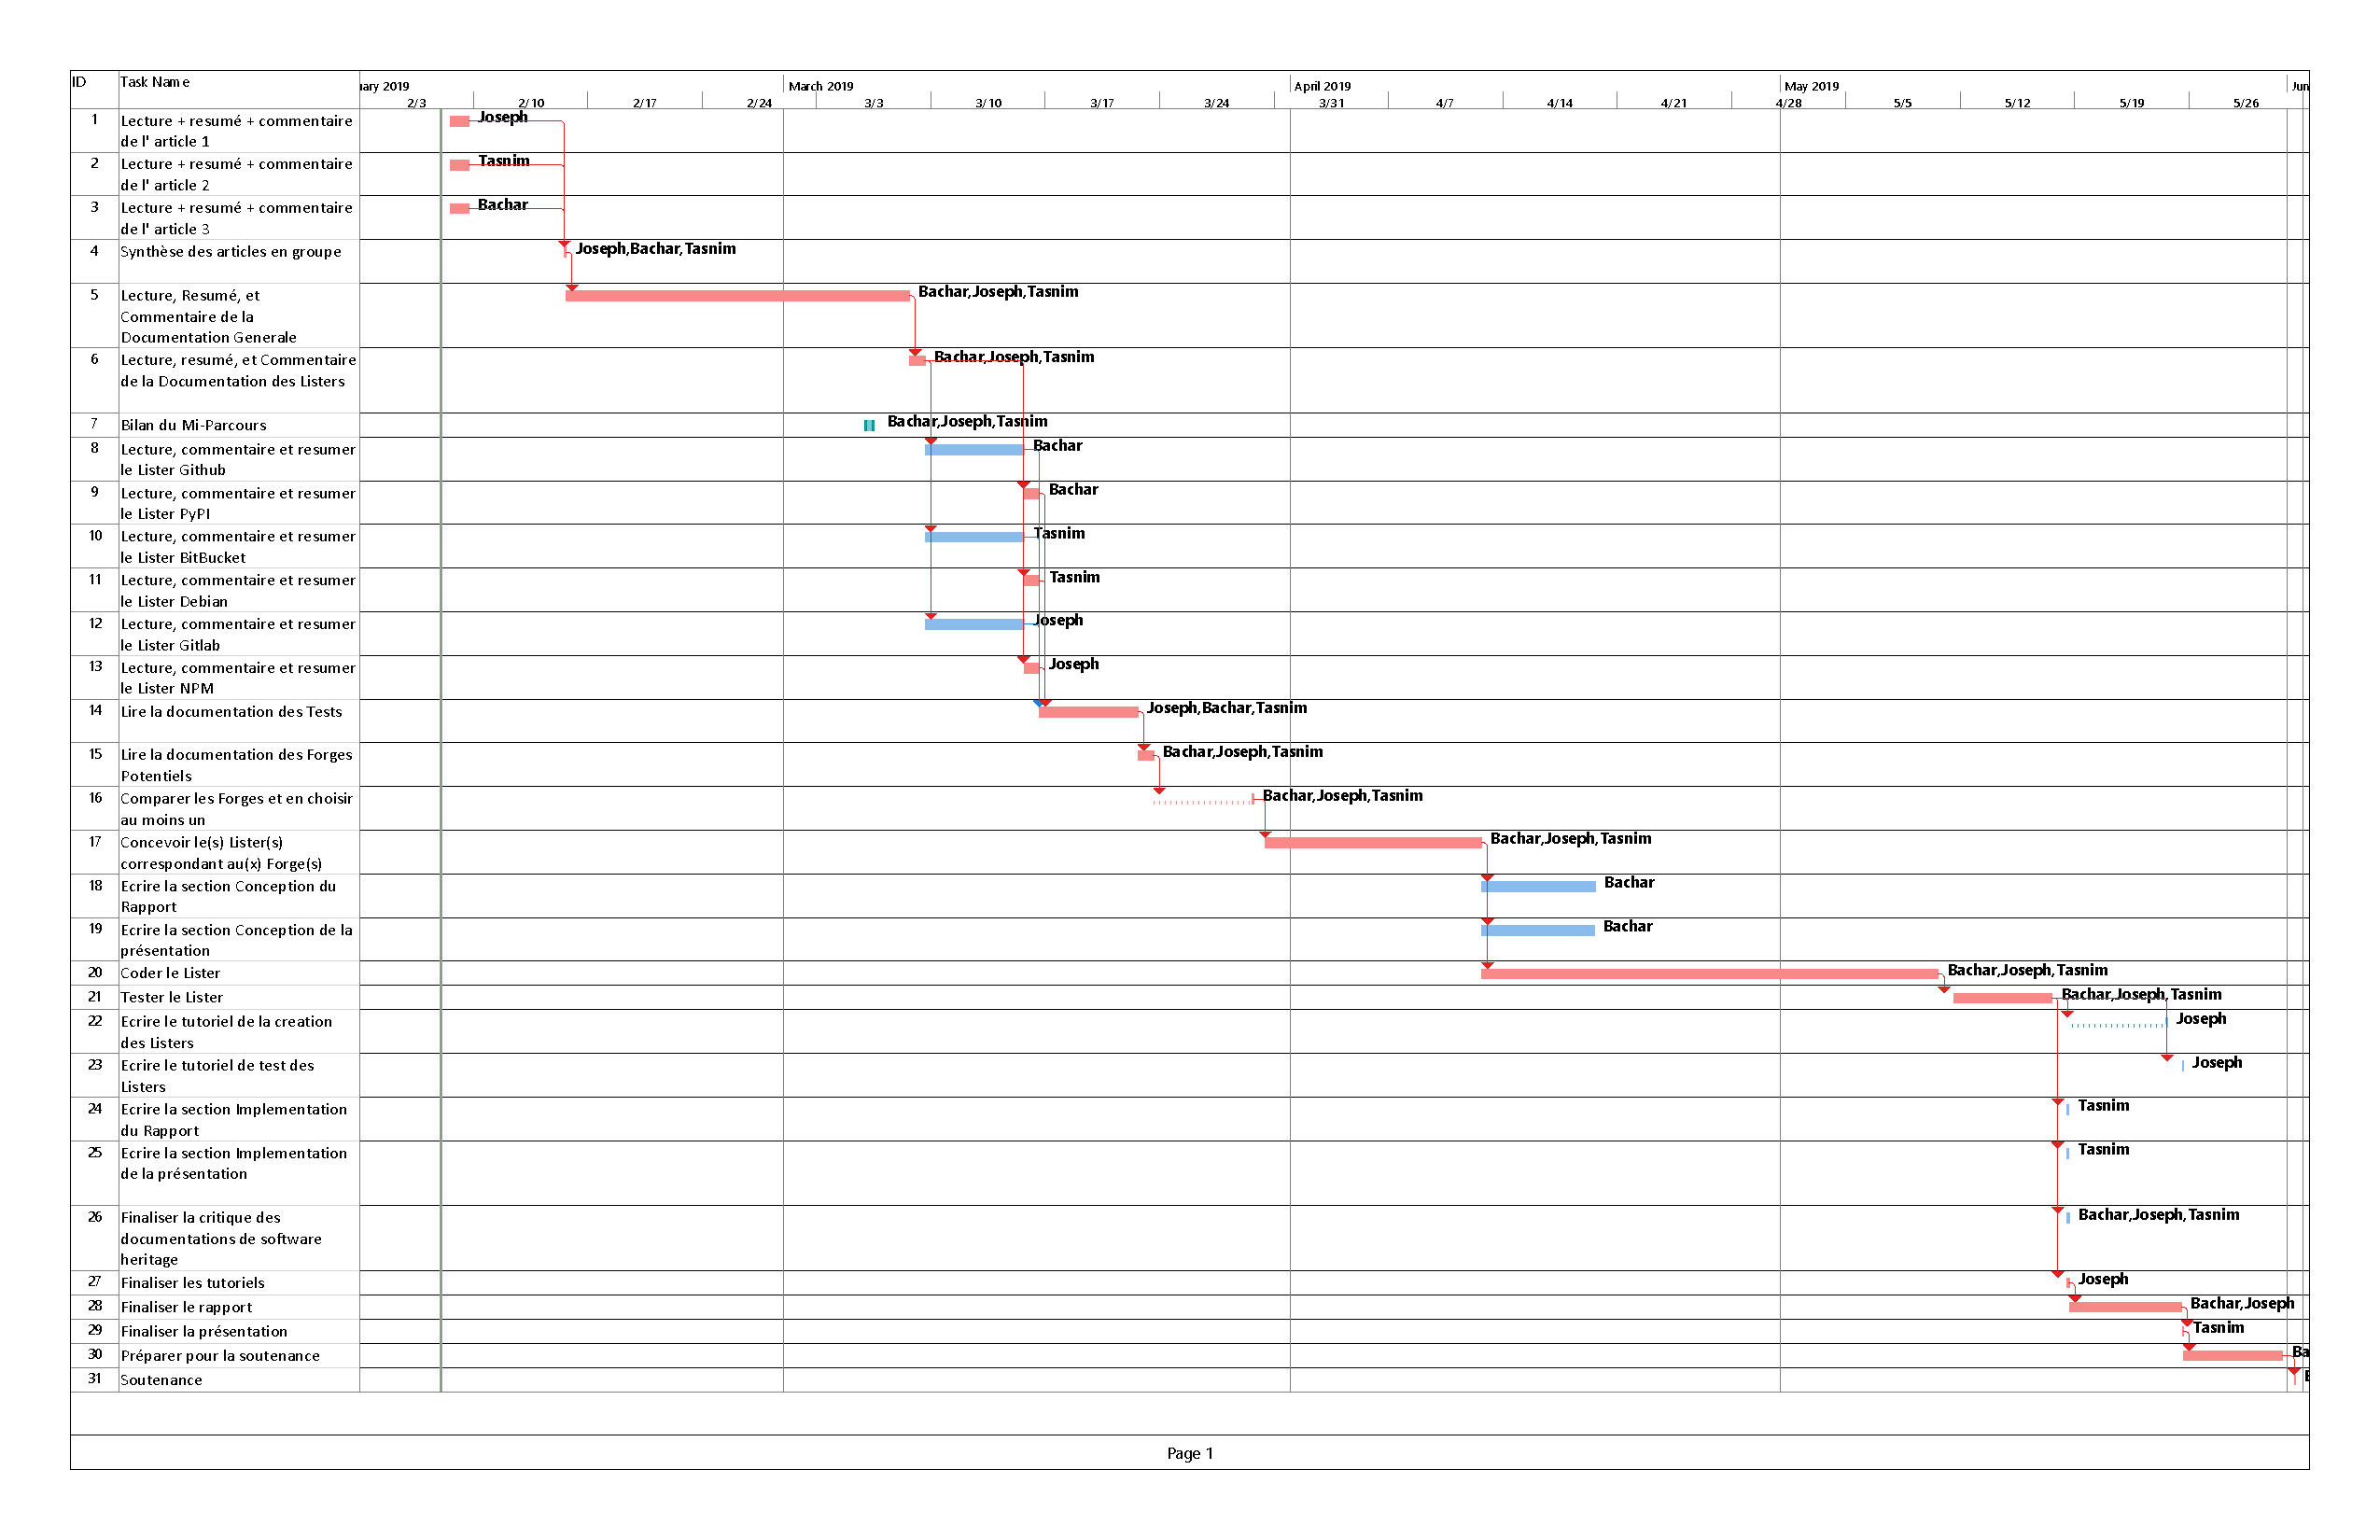
\includepdf{pdf/feuille_de_route.pdf}
\end{figure}

\end{document}
